\documentclass{article}

\usepackage{fancyhdr}
\usepackage{extramarks}
\usepackage{amsmath}
\usepackage{amsthm}
\usepackage{amsfonts}
\usepackage{tikz}
\usepackage[plain]{algorithm}
\usepackage{algpseudocode}
\usepackage{graphicx}
\usepackage{xcolor}
\usepackage[dvipsnames]{xcolor}

\usetikzlibrary{automata,positioning}

%
% Basic Document Settings
%

\topmargin=-0.45in
\evensidemargin=0in
\oddsidemargin=0in
\textwidth=6.5in
\textheight=9.0in
\headsep=0.25in

\linespread{1.1}

\pagestyle{fancy}
%\lhead{\hmwkAuthorName}
%\chead{\hmwkClass\ (\hmwkClassInstructor\ \hmwkClassTime): \hmwkTitle}
\rhead{\firstxmark}
\lfoot{\lastxmark}
\cfoot{\thepage}

\renewcommand\headrulewidth{0.4pt}
\renewcommand\footrulewidth{0.4pt}

\setlength\parindent{0pt}

%
% Create Problem Sections
%

\newcommand{\enterProblemHeader}[1]{
    \nobreak\extramarks{}{Problem \arabic{#1} continued on next page\ldots}\nobreak{}
    \nobreak\extramarks{Problem \arabic{#1} (continued)}{Problem \arabic{#1} continued on next page\ldots}\nobreak{}
}

\newcommand{\exitProblemHeader}[1]{
    \nobreak\extramarks{Problem \arabic{#1} (continued)}{Problem \arabic{#1} continued on next page\ldots}\nobreak{}
    \stepcounter{#1}
    \nobreak\extramarks{Problem \arabic{#1}}{}\nobreak{}
}

\setcounter{secnumdepth}{0}
\newcounter{partCounter}
\newcounter{homeworkProblemCounter}
\setcounter{homeworkProblemCounter}{1}
\nobreak\extramarks{Problem \arabic{homeworkProblemCounter}}{}\nobreak{}

%
% Homework Problem Environment
%
% This environment takes an optional argument. When given, it will adjust the
% problem counter. This is useful for when the problems given for your
% assignment aren't sequential. See the last 3 problems of this template for an
% example.
%
\newenvironment{homeworkProblem}[1][-1]{
    \ifnum#1>0
        \setcounter{homeworkProblemCounter}{#1}
    \fi
    \section{Problem \arabic{homeworkProblemCounter}}
    \setcounter{partCounter}{1}
    \enterProblemHeader{homeworkProblemCounter}
}{
    \exitProblemHeader{homeworkProblemCounter}
}

%
% Homework Details
%   - Title
%   - Due date
%   - Class
%   - Section/Time
%   - Instructor
%   - Author
%

\newcommand{\hmwkTitle}{Exercise\ \#8}
\newcommand{\hmwkDueDate}{September 22, 2025}
\newcommand{\hmwkClass}{Advanced Econometrics}
\newcommand{\hmwkClassTime}{}
\newcommand{\hmwkClassInstructor}{Professor Paulo Parente}
\newcommand{\hmwkAuthorName}{\textbf{Amy Qian}}

%
% Title Page
%

\title{
    \vspace{2in}
    \textmd{\textbf{\hmwkClass:\ \hmwkTitle}}\\
    \normalsize\vspace{0.1in}\small{\hmwkDueDate}\\
    \vspace{0.1in}\large{\textit{\hmwkClassInstructor\ \hmwkClassTime}}
    \vspace{3in}
}

\author{\hmwkAuthorName}
\date{}

\renewcommand{\part}[1]{\textbf{\large Part \Alph{partCounter}}\stepcounter{partCounter}\\}

%
% Various Helper Commands
%

% Useful for algorithms
\newcommand{\alg}[1]{\textsc{\bfseries \footnotesize #1}}

% For derivatives
\newcommand{\deriv}[1]{\frac{\mathrm{d}}{\mathrm{d}x} (#1)}

% For partial derivatives
\newcommand{\pderiv}[2]{\frac{\partial}{\partial #1} (#2)}

% Integral dx
\newcommand{\dx}{\mathrm{d}x}

% Alias for the Solution section header
\newcommand{\solution}{\textbf{\large Solution}}

% Probability commands: Expectation, Variance, Covariance, Bias
\newcommand{\E}{\mathrm{E}}
\newcommand{\Var}{\mathrm{Var}}
\newcommand{\Cov}{\mathrm{Cov}}
\newcommand{\Bias}{\mathrm{Bias}}

\begin{document}

\maketitle

\pagebreak

\begin{homeworkProblem}
    Obtain a non-parametric estimate of the density of lhhexp1.
    Compare the bandwith used by STATA with the one suggested by Silverman's rule of thumb.\\

    \textbf{STATA}
    \\
    \textcolor{Magenta}{kdensity lhhexp1, kernel(gaussian)}
    \\
    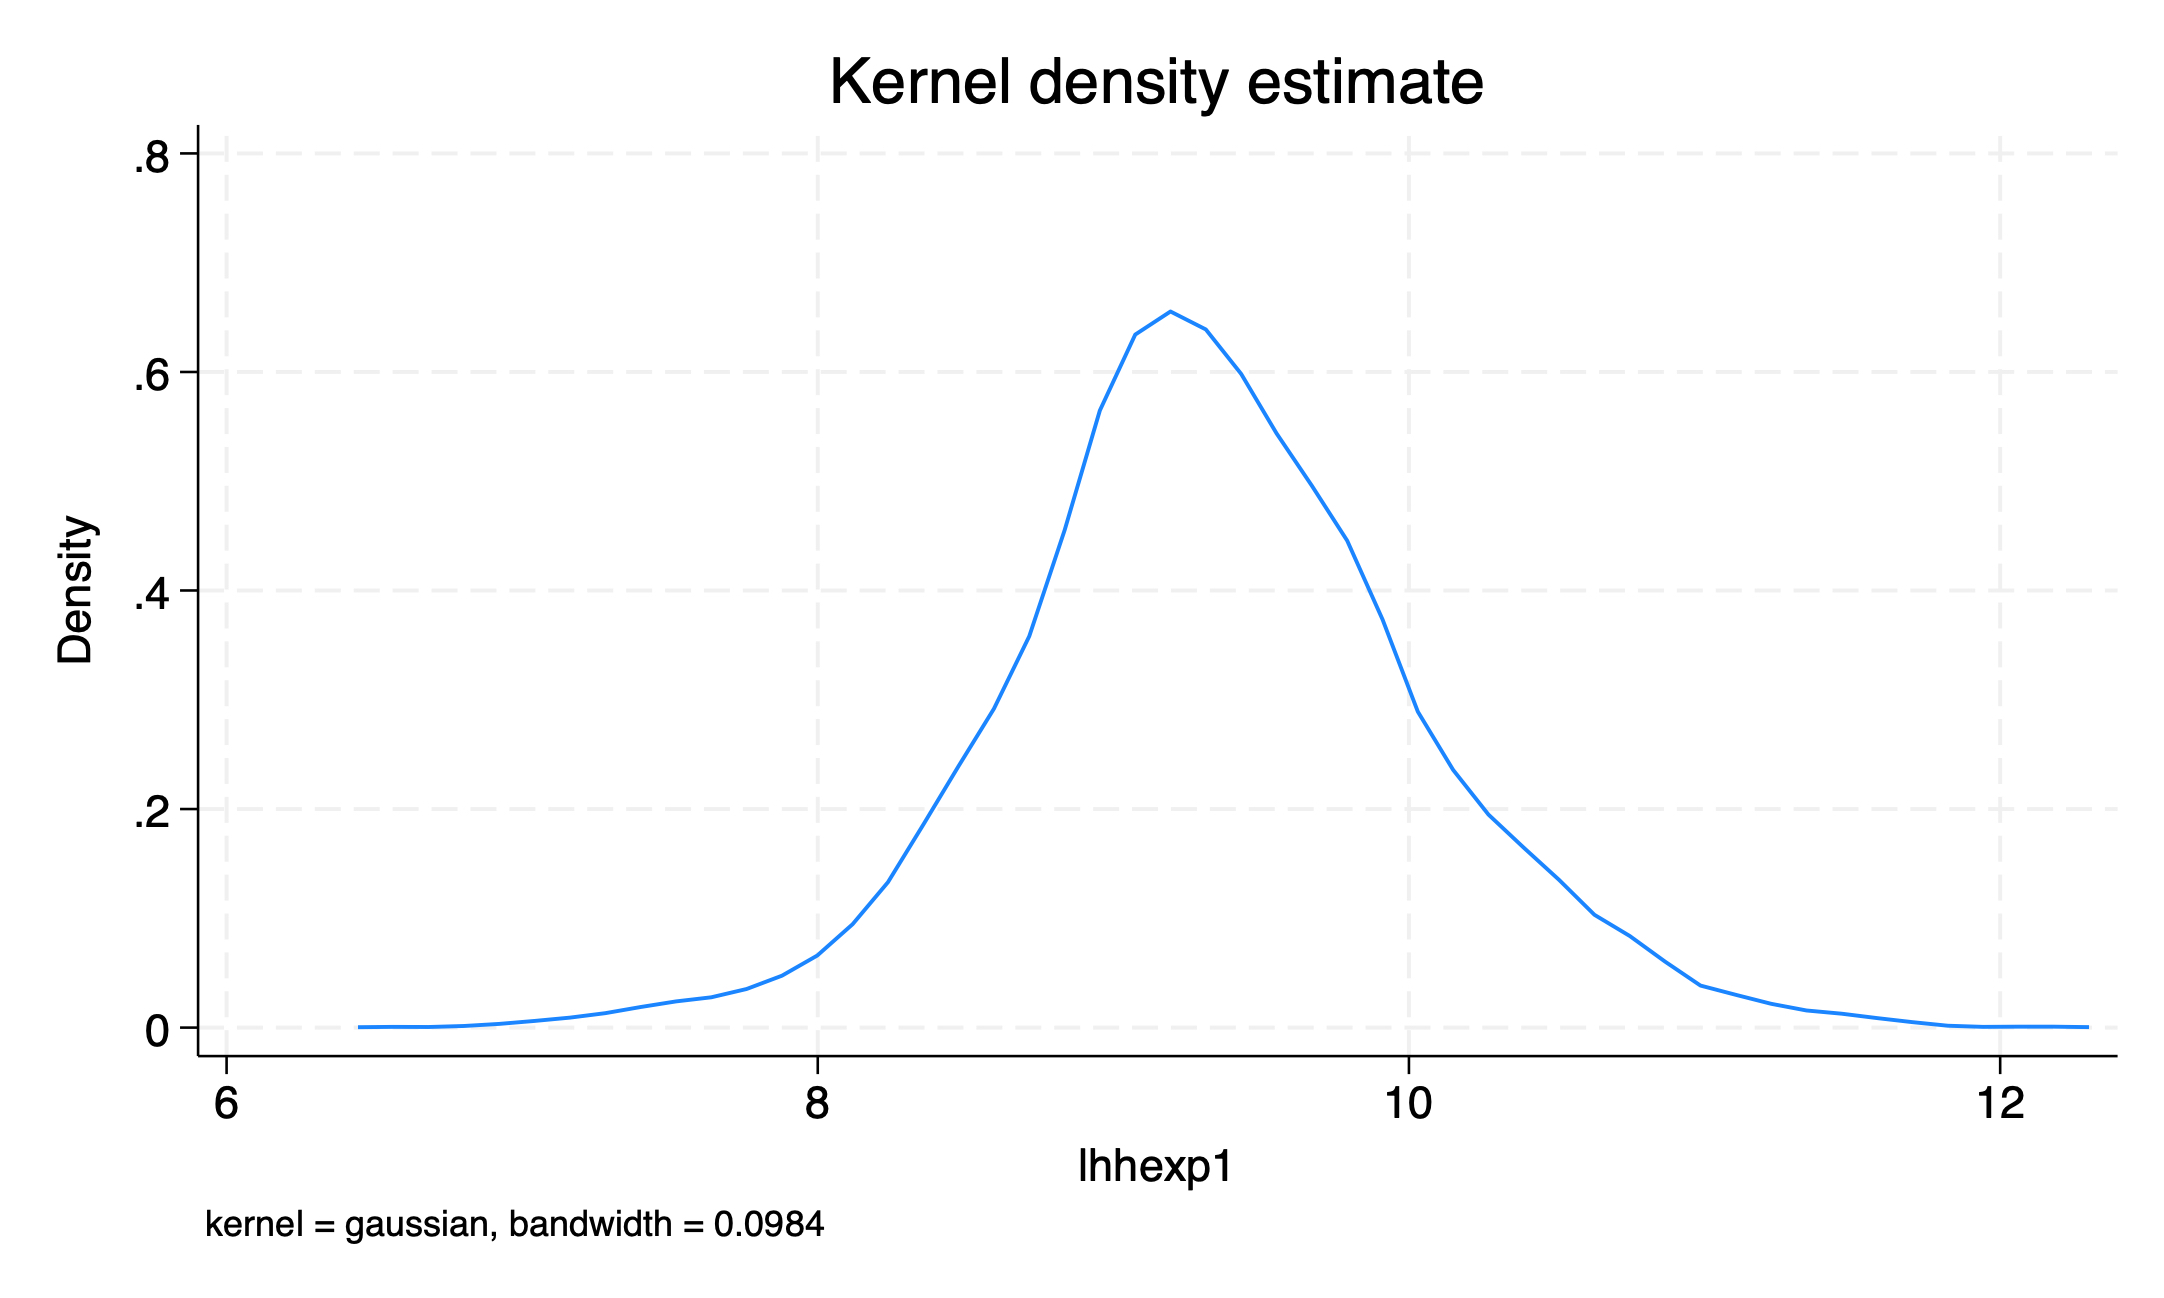
\includegraphics[scale=0.1]{Image/1.jpg}
    \\
    Bandwith used by STATA: 0.0984
    \\
    
    \textbf{Silverman's Rule of Thumb}
    \\
    \textcolor{Magenta}{sum lhhexp1, d}
    \\

    This gives us
    \begin{itemize}
        \item Standard deviation: 0.6877458
        \item n: 5,999
        \item IQR: 9.759566 - 8.919547 = 0.840019
    \end{itemize}
    To calculate Silverman's bandwith, we use the formula:
    $h = \min(\sigma, \frac{IQR}{1.34}) \frac{0.9}{n^{-1/5}}$
    \\
    Plugging in our values, we get:
    \begin{itemize}
        \item \textcolor{Magenta}{display ((.6877458*0.9)/5999\^{}(0.2))} = .10865624
        \item \textcolor{Magenta}{display (((9.759566 - 8.919547)/1.34*0.9)/5999\^{}(0.2))} = .09904009
    \end{itemize}
    So the bandwidth suggested by Silverman's rule of thumb is 0.09904009,
    which is very close to the bandwidth used by STATA.
\end{homeworkProblem}

\begin{homeworkProblem}
    Repeat the previous exercise using different kernels.
    \\

    \textbf{Rectangular Kernel}\\
    \textcolor{Magenta}{kdensity lhhexp1, kernel(rec)}
    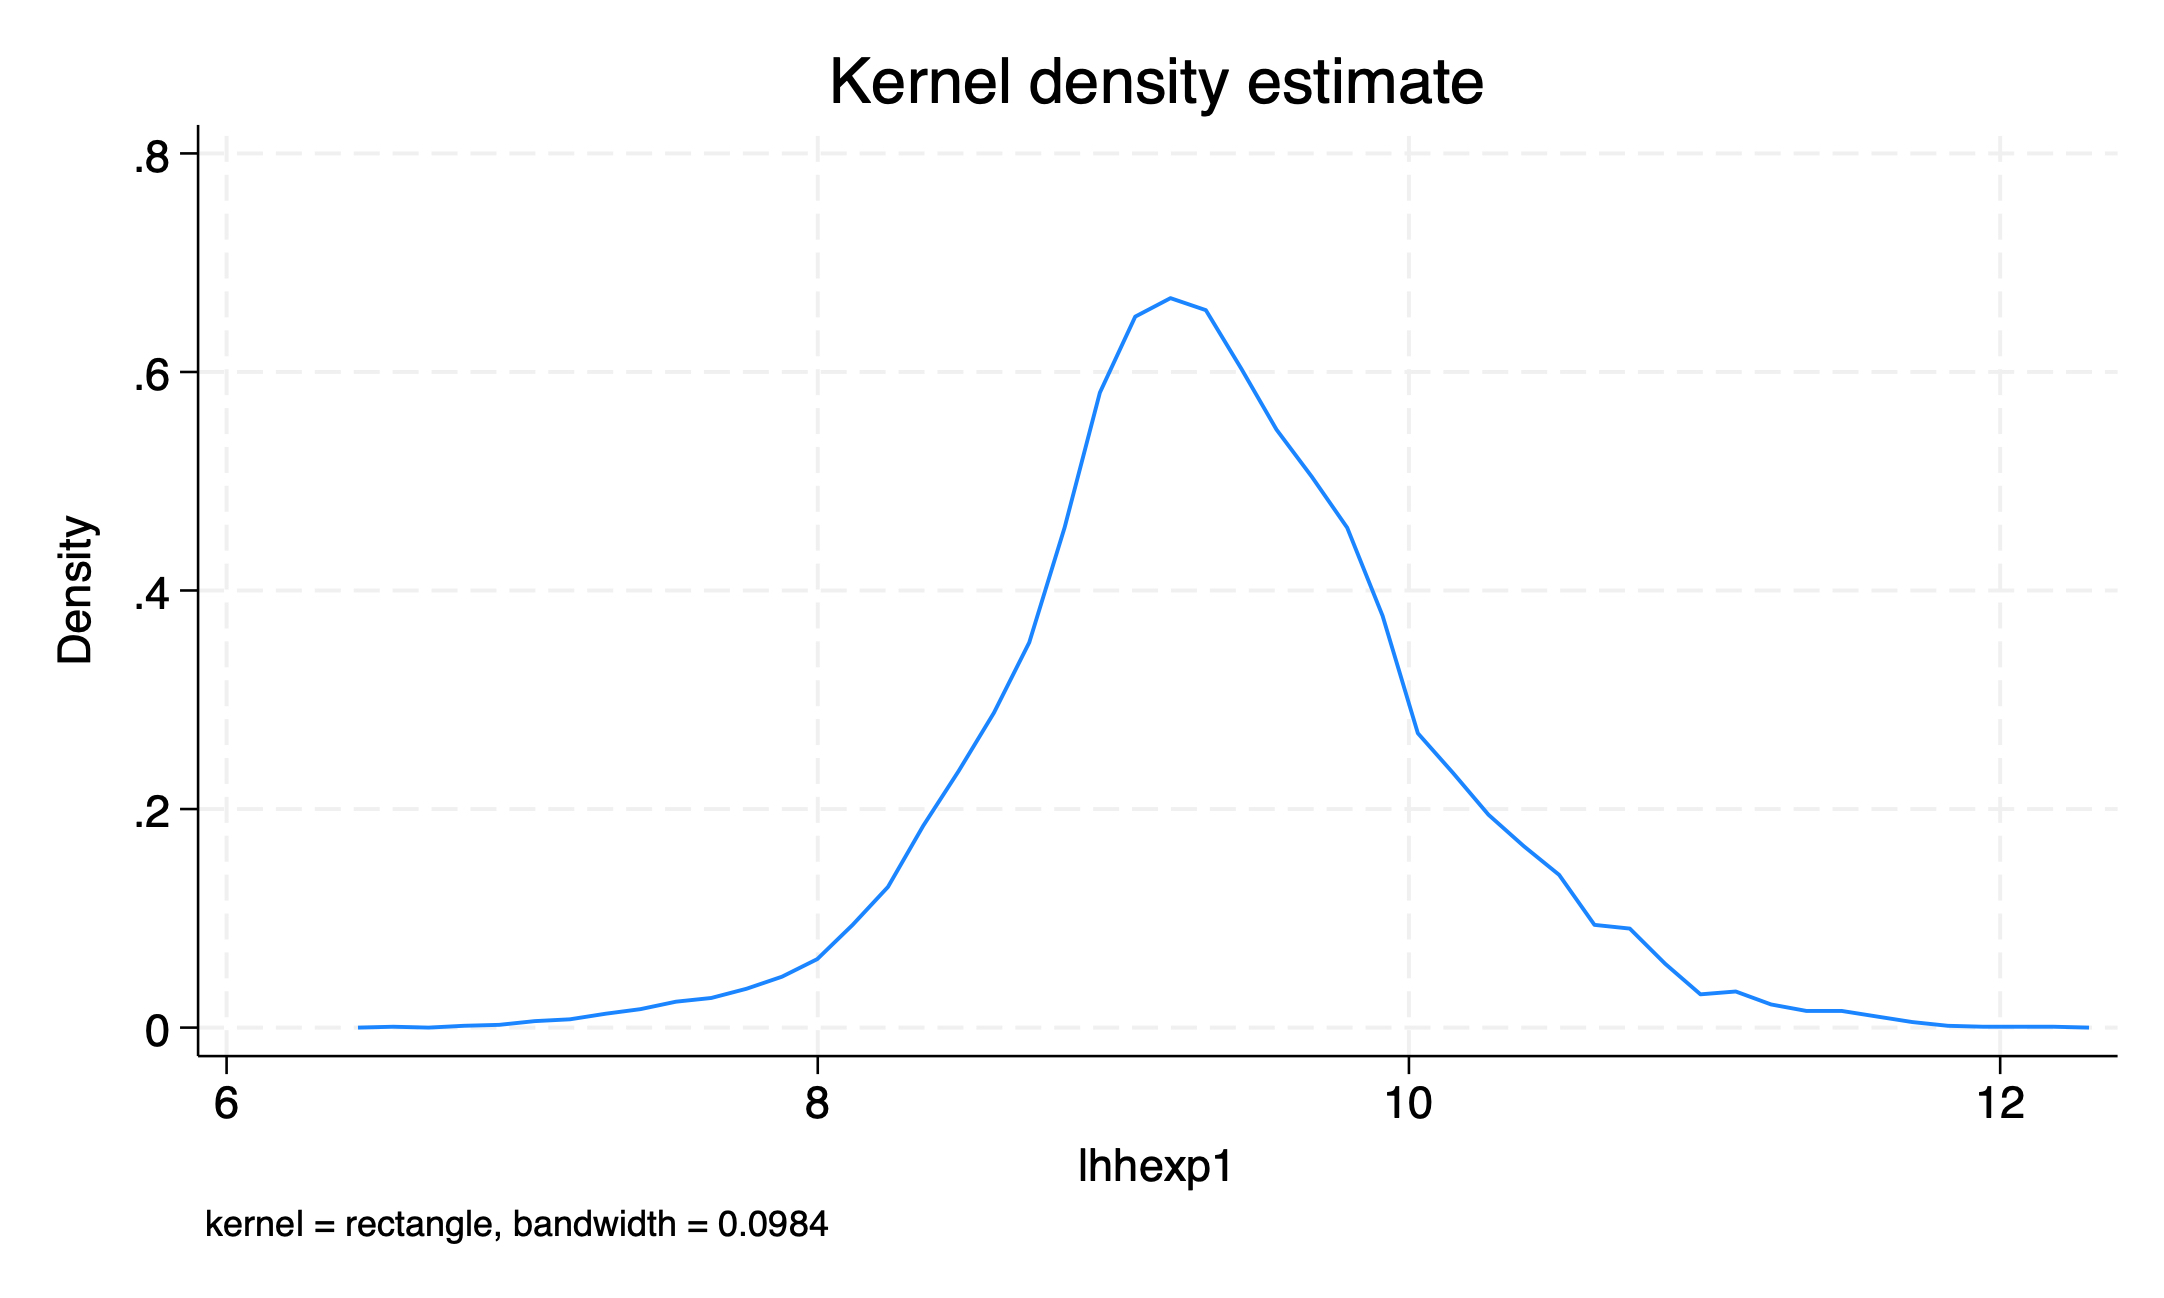
\includegraphics[scale=0.1]{Image/2.jpg}\\
    This is less smooth than the Gaussian kernel.
    \\

    \textbf{Parzan Kernel}\\
    \textcolor{Magenta}{kdensity lhhexp1, kernel(parz)}
    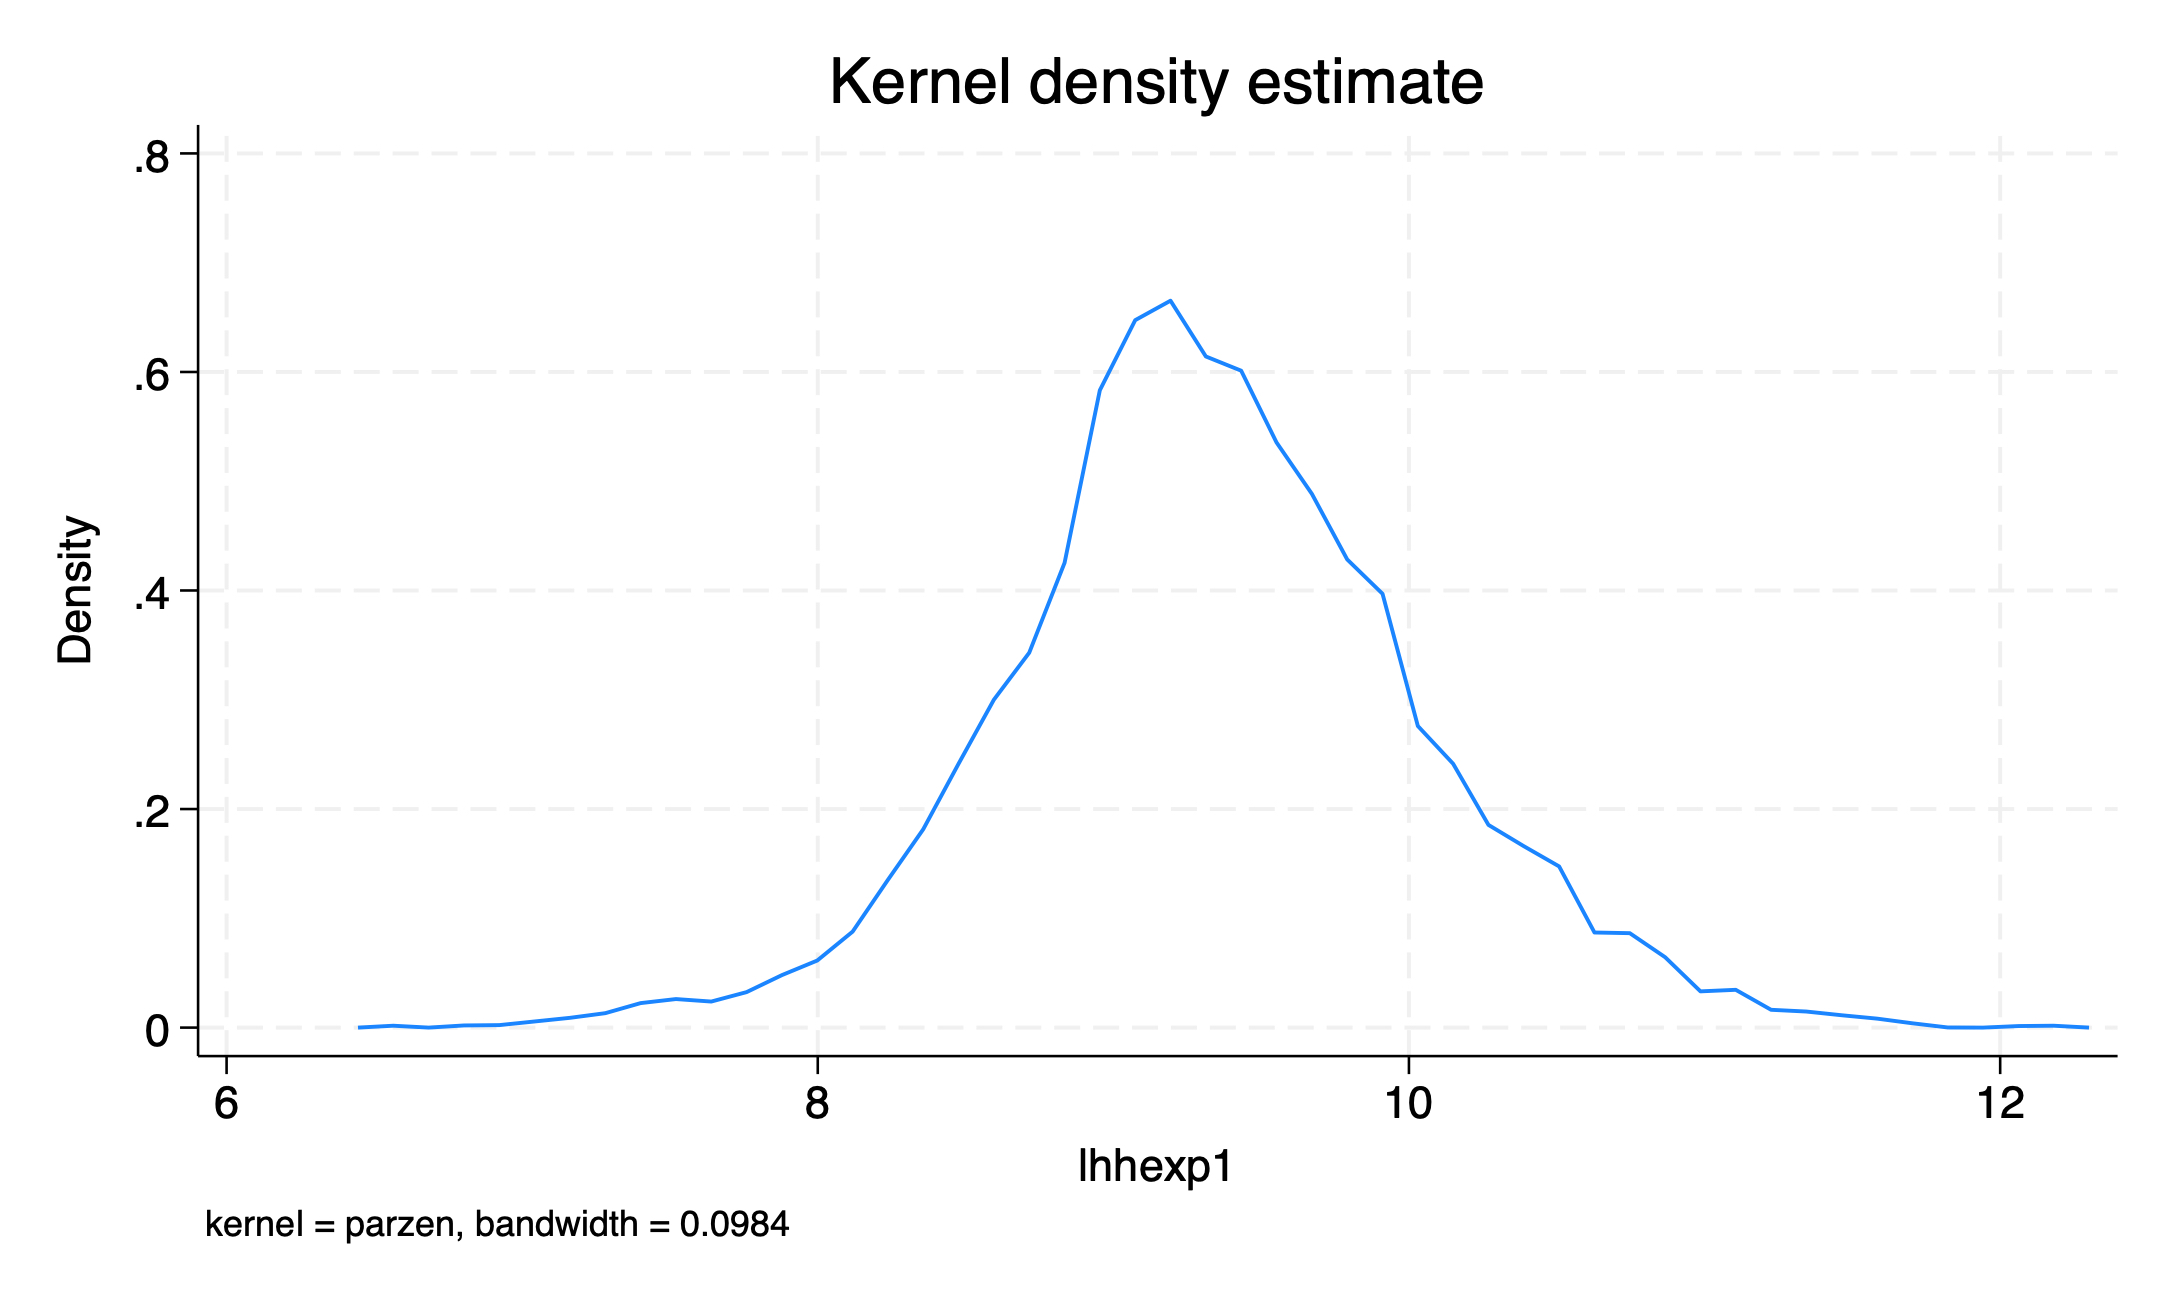
\includegraphics[scale=0.1]{Image/3.jpg}\\
    This is also less smooth than the Gaussian kernel.
    \\

    \textbf{Gaussian with different bandwidth}\\
    \textcolor{Magenta}{kdensity lhhexp1, kernel(gaussian) bwidth(0.002)}
    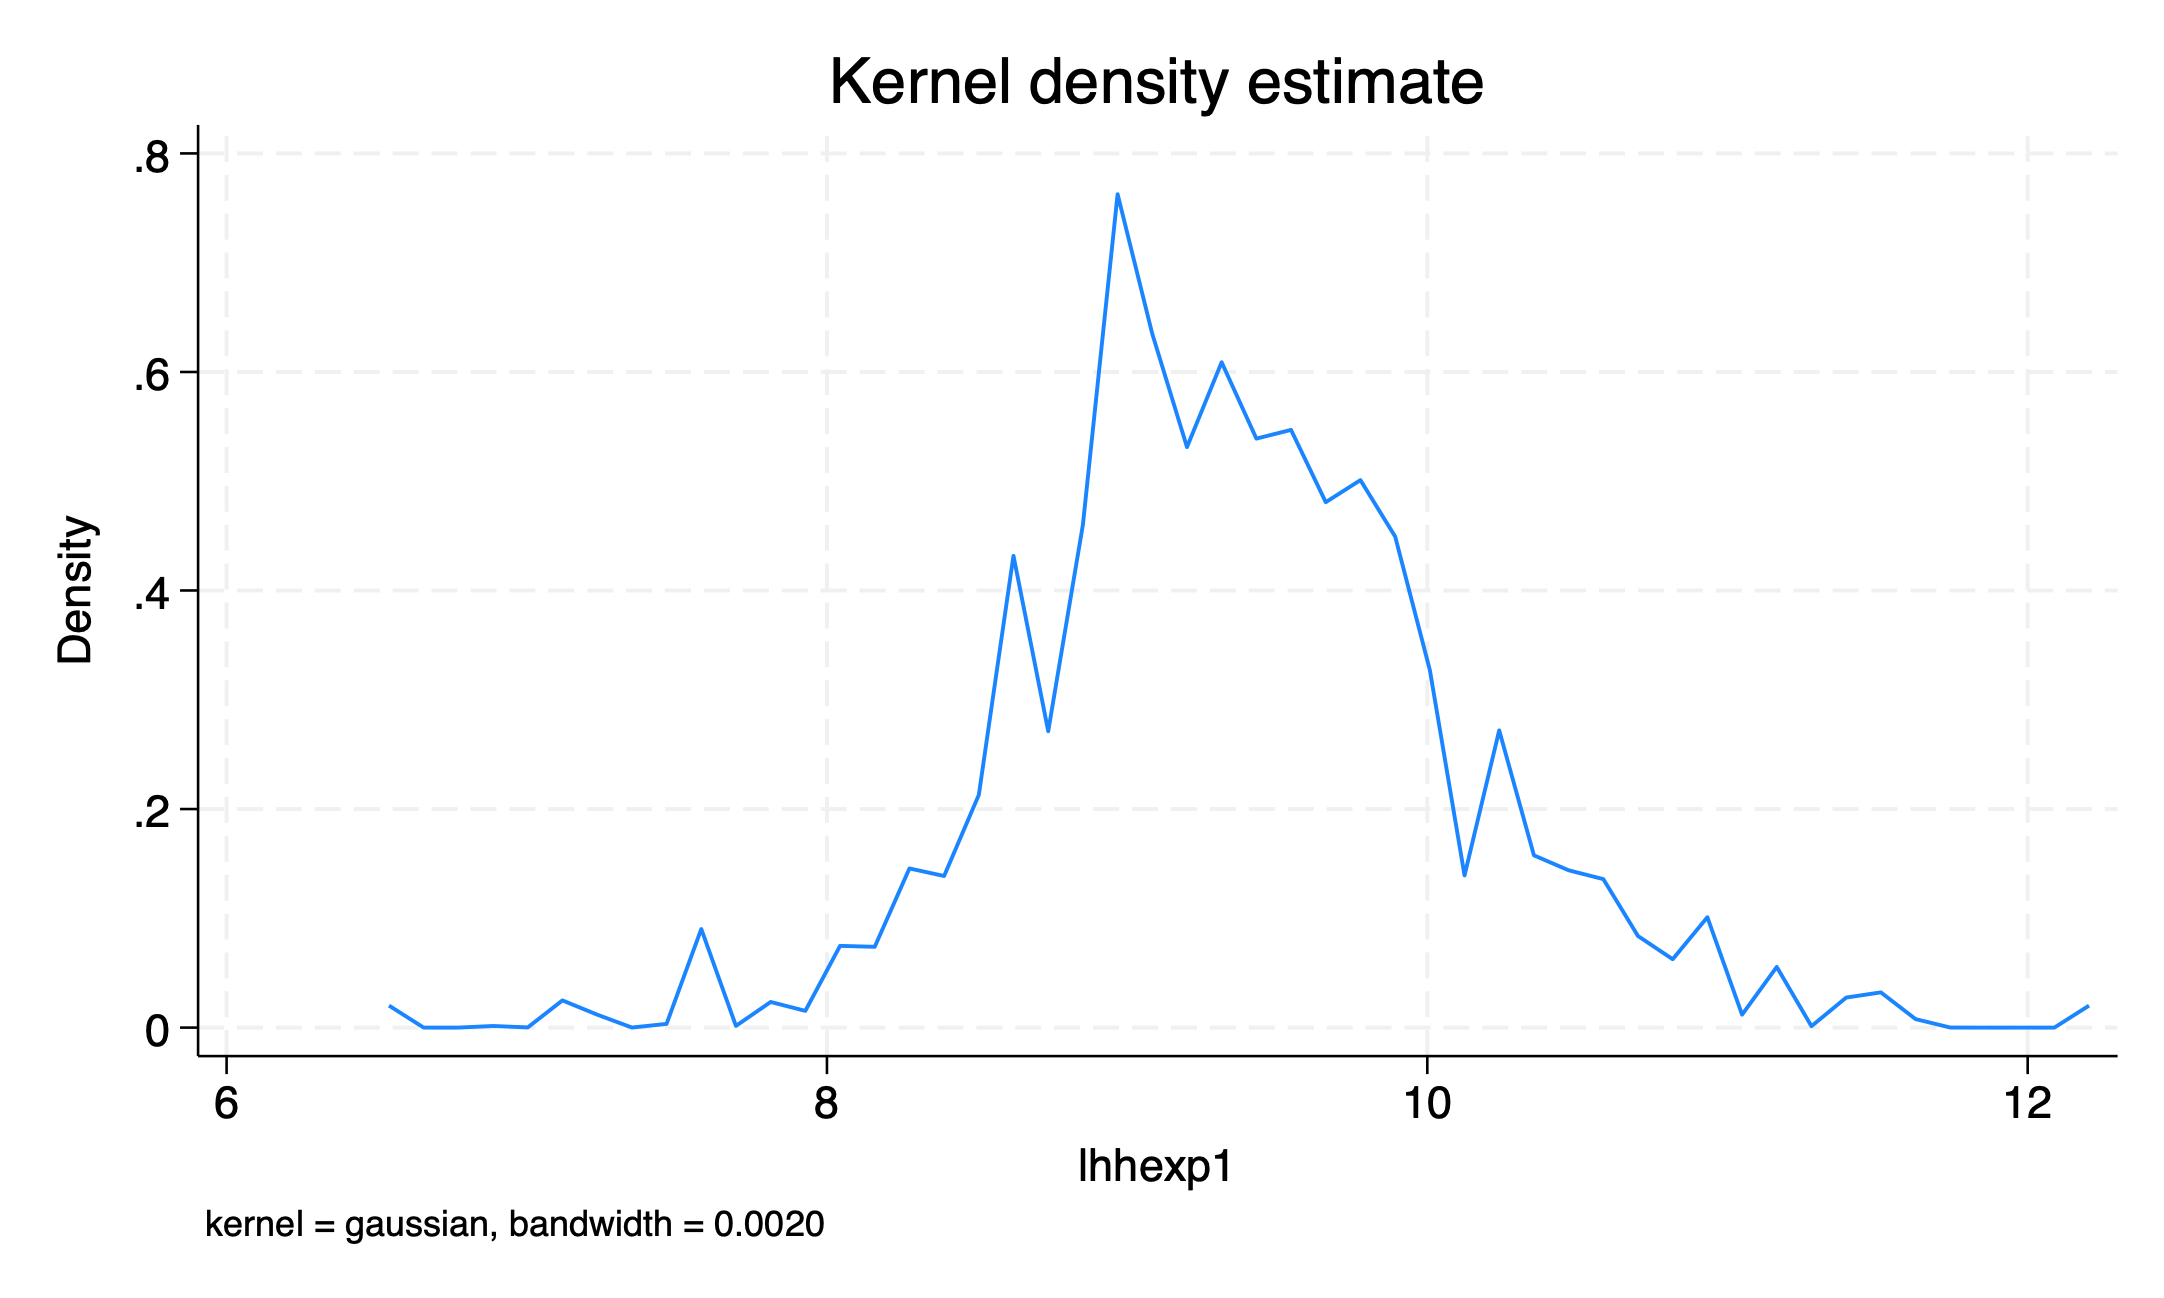
\includegraphics[scale=0.1]{Image/4.jpg}\\
    \textcolor{Magenta}{kdensity lhhexp1, kernel(gaussian) bwidth(1)}
    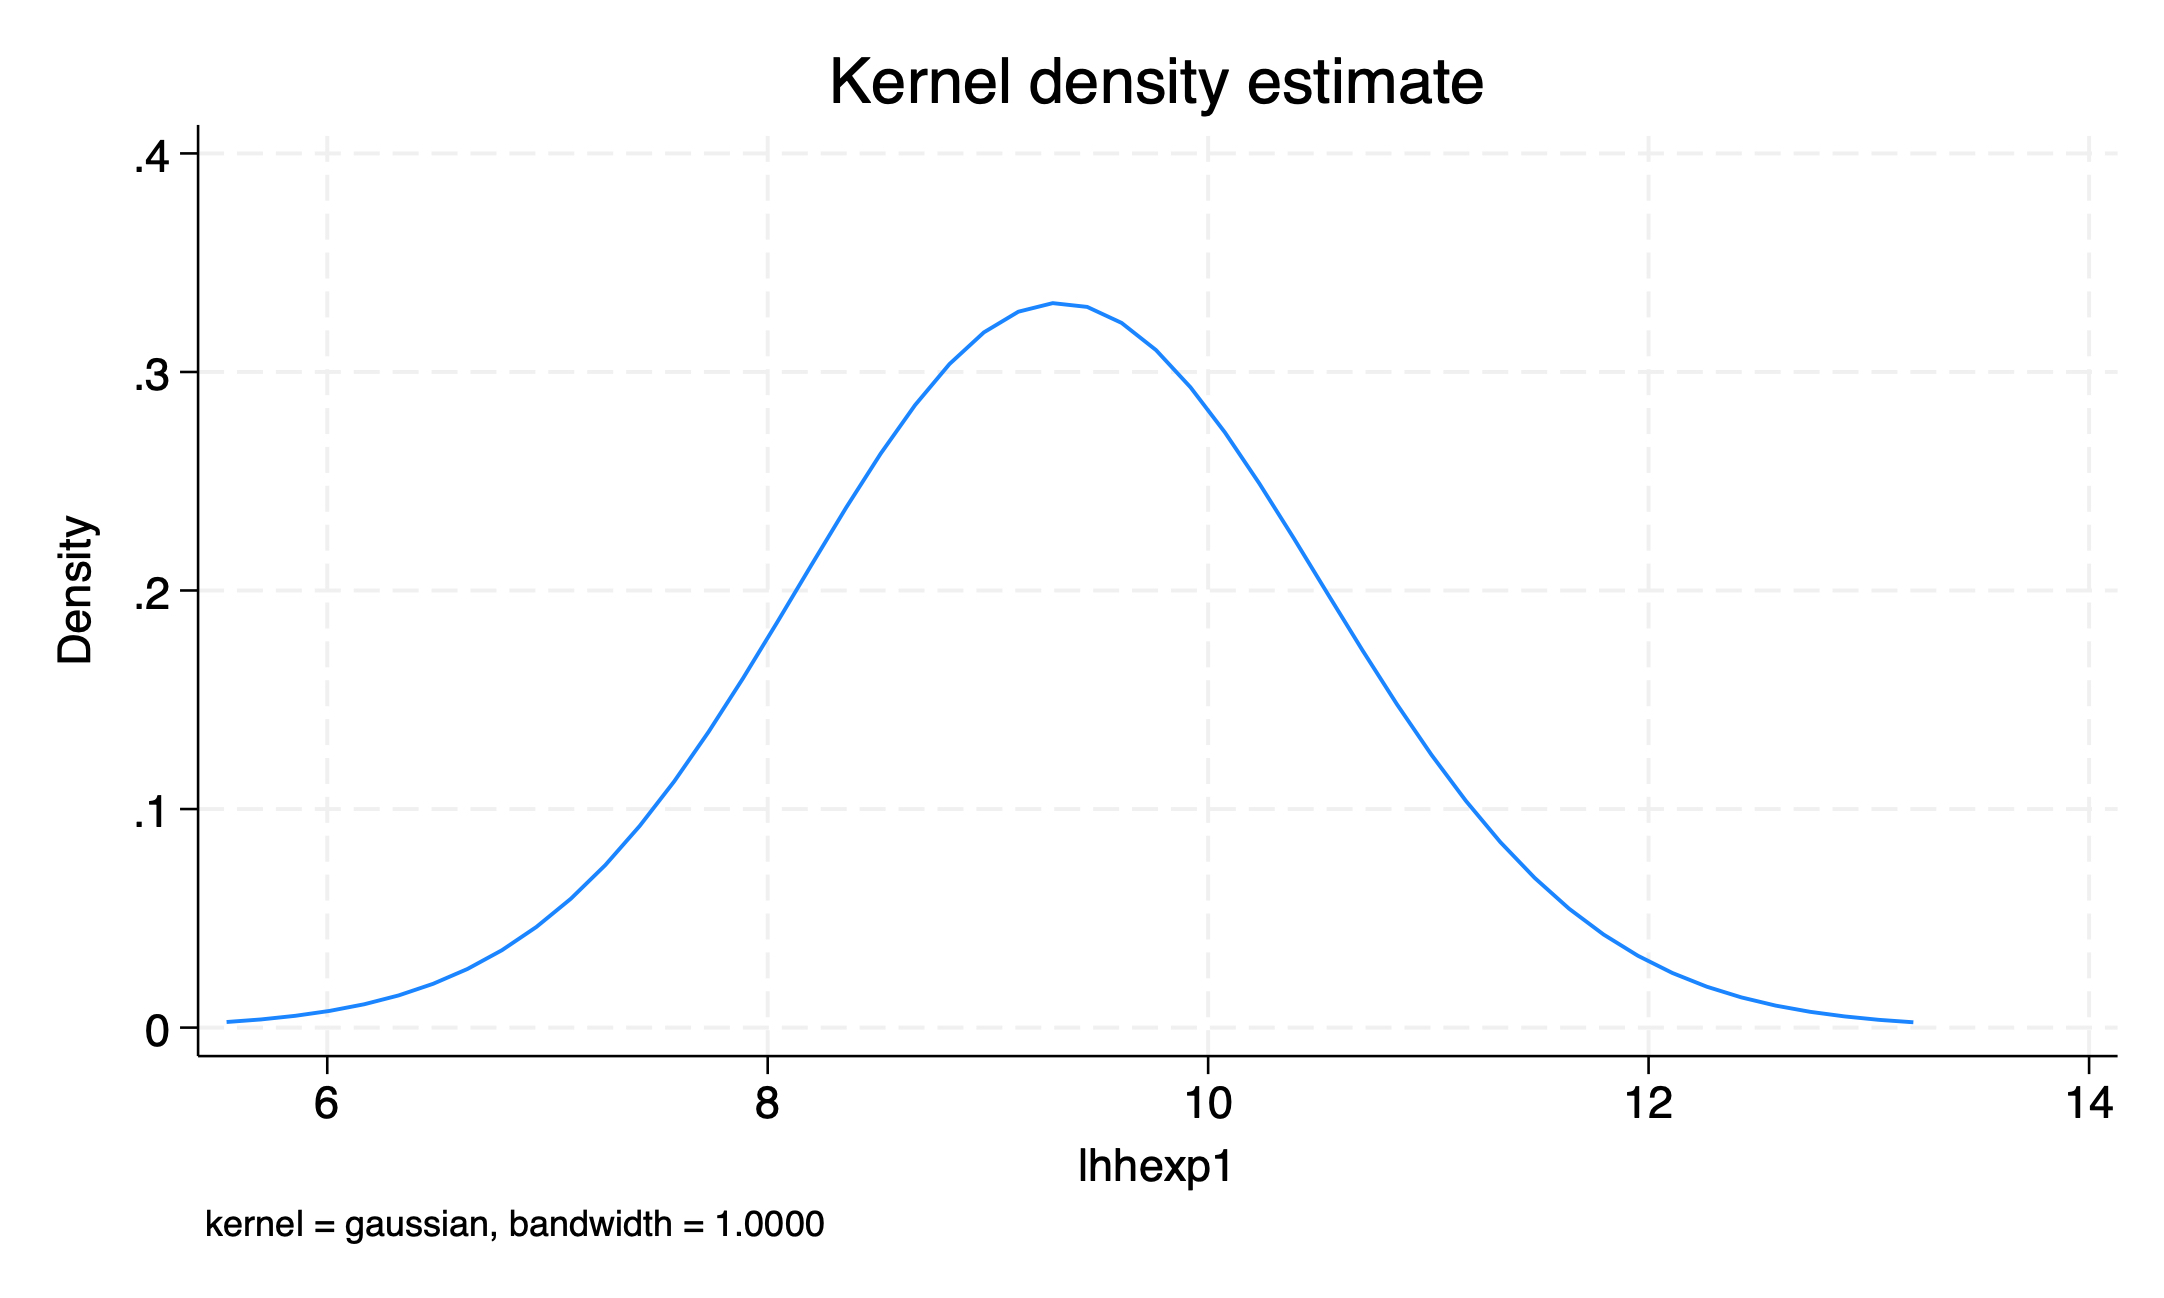
\includegraphics[scale=0.1]{Image/5.jpg}\\

    In general, the bandwith is more important than the kernel.
    We want it to be smooth enough but not too smooth that we miss important
    features of the data.
\end{homeworkProblem}

\begin{homeworkProblem}
    Obtain the Nadaraya-Watson estimator of the conditional expectation of lnrlfood,
    the log household expenditure on food, given lhhexp1.
    Does the result suggest that this conditional expectation is linear?
    \\

    \solution
    \\

    We wan to estimate $E[y_i | x_i] = m(x_i)$ where $y_i$ is lnrlfood.

    \textcolor{Magenta}{lpoly lnrlfood lhhexp1}
    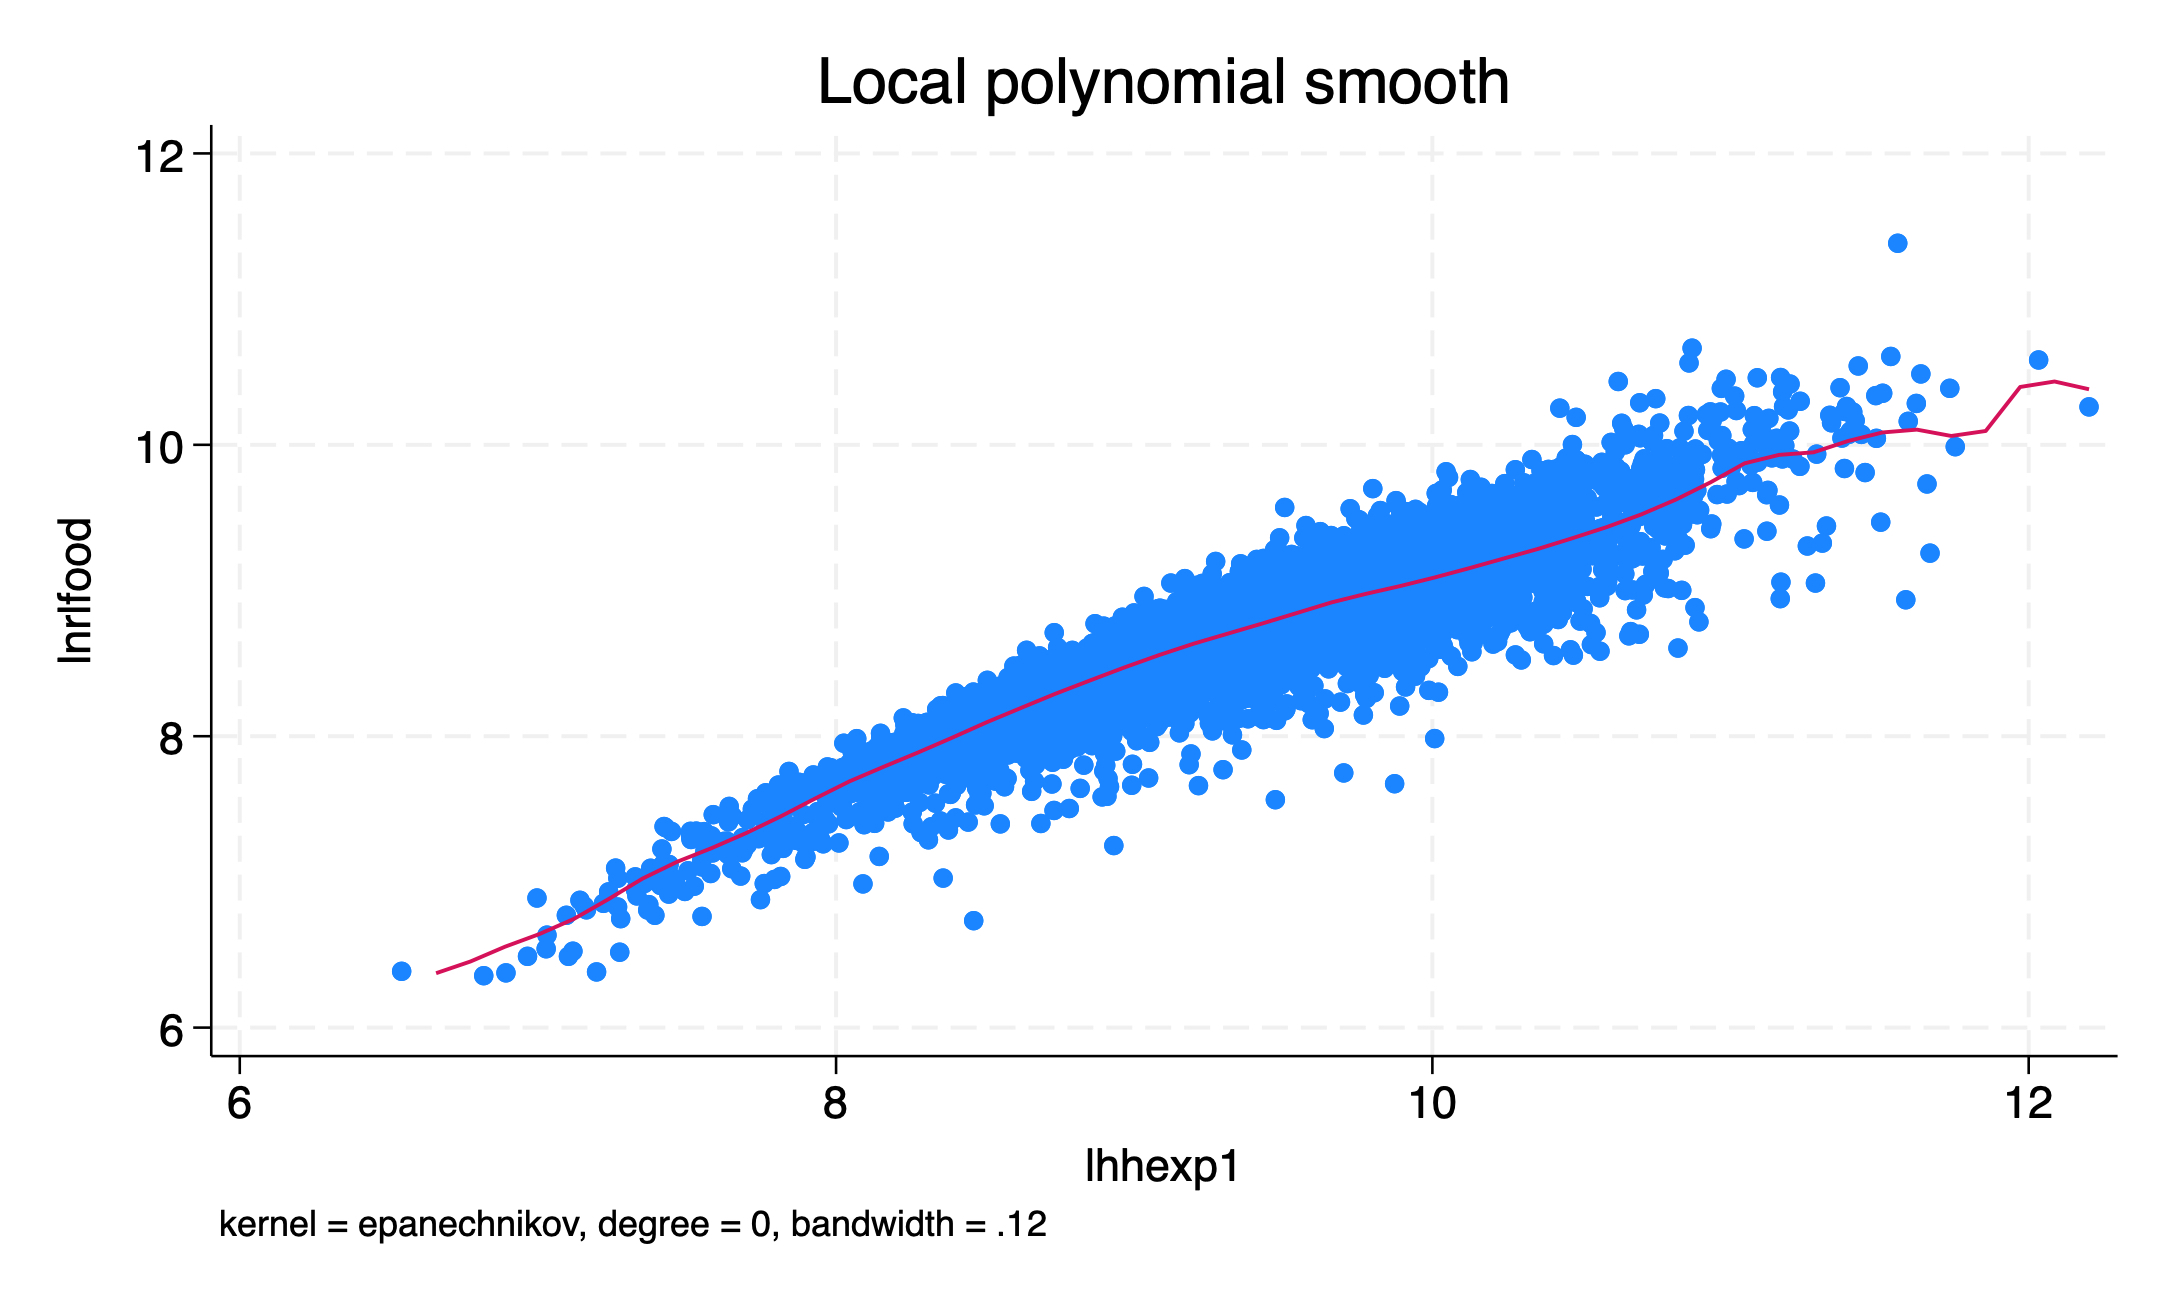
\includegraphics[scale=0.1]{Image/6.jpg}\\
    Blue dots are the data points,
    the red line is the estimated conditional expectation (the function).
    Could be linear looking at the graph, but not exactly linear.

\end{homeworkProblem}

\begin{homeworkProblem}
    Using OLS, estimate a regression of lnrlfood on lhhexp1, age and its square.
    Is the effect of age linear?
    \\

    \solution
    \\

    First generate the new variable age squared.
    \\
    \textcolor{Magenta}{gen age2 = age\^{}2}
    \\
    Then run the OLS regression using robust standard errors
    to control for heteroskedasticity.
    \\
    \textcolor{Magenta}{reg lnrlfood lhhexp1 age age2, r}
    \\
    We want to test the null hypothesis that the effect of age is linear,
    which is equivalent to testing if the coefficient of age2 is zero.
    \\
    \centerline{$H_0: \beta_{\text{age2}} = 0$ vs. $H_a: \beta_{\text{age2}} \neq 0$}
    \\
    From the regression output, we see that the p-value is 0.000,
    which is less than 0.05, so we reject $H_0$ in favor of $H_1$ at 5\% confidence level.

\end{homeworkProblem}

\begin{homeworkProblem}
    Use the partially linear estimator to estimate in the following model:
    $\text{lnrlfood}_i = \beta\text{lhhexp1}_i + g(\text{age}_i)+u_i$
    \\

    \solution
    \\

    $G(\cdot)$ is now an unknown function.
    \\
    Get the estimates
    \begin{itemize}
        \item $E[y_i|\text{age}_i] \Rightarrow \text{foodage}$.
        \textcolor{Magenta}{lpoly lnrlfood age, generate(foodage) at (age)}
        \item $E[x_i|\text{age}_i] \Rightarrow \text{expage}$.
        \textcolor{Magenta}{lpoly lhhexp1 age, generate(expage) at (age)}
    \end{itemize}
    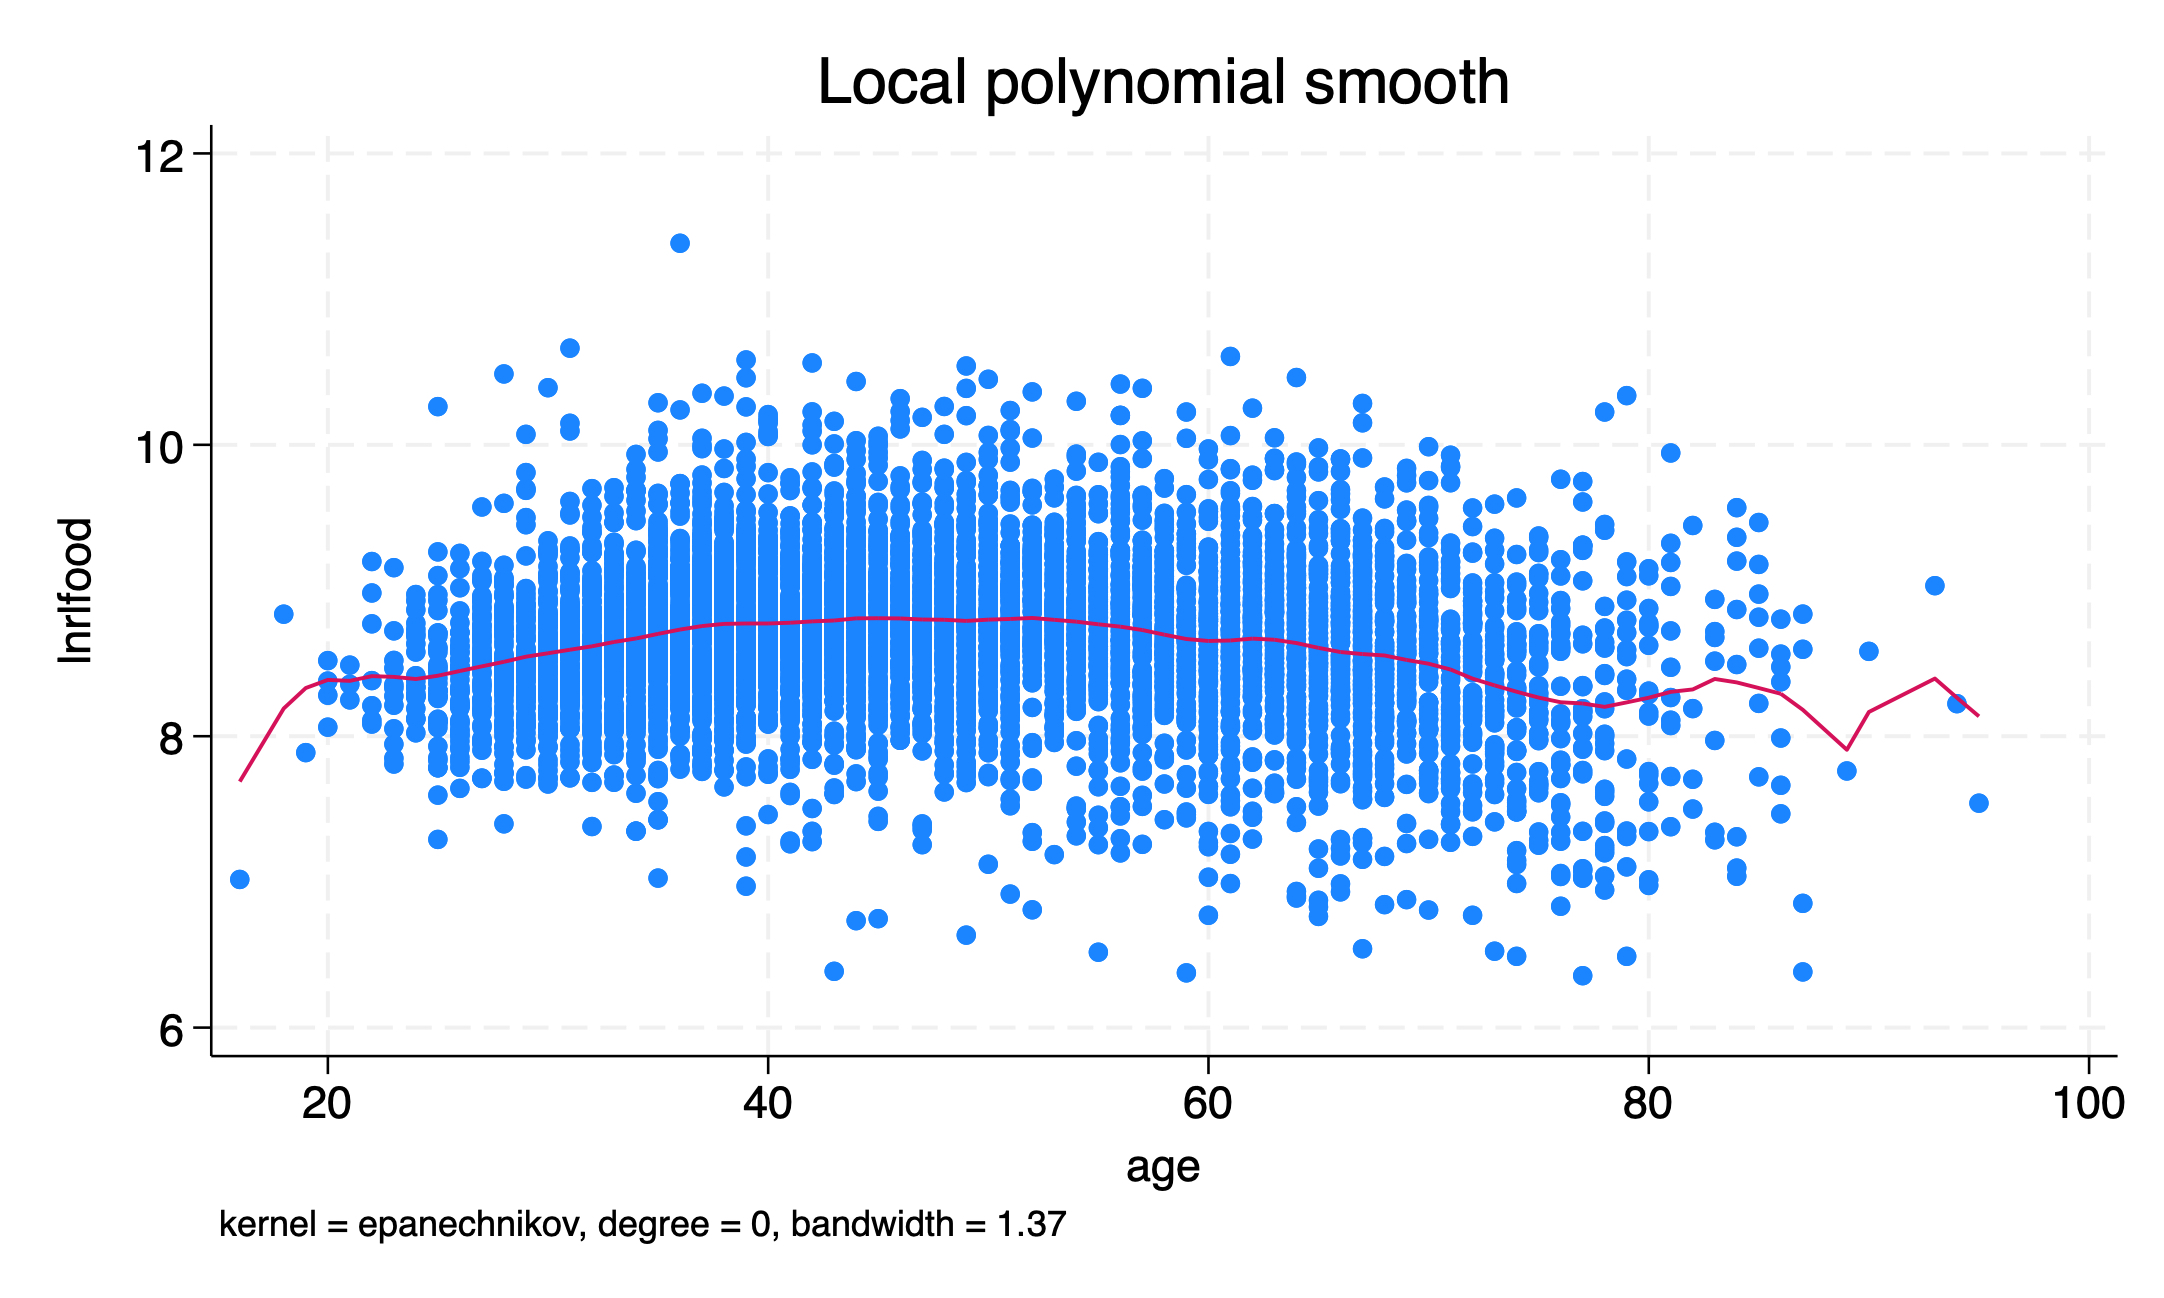
\includegraphics[scale=0.1]{Image/7.jpg}
    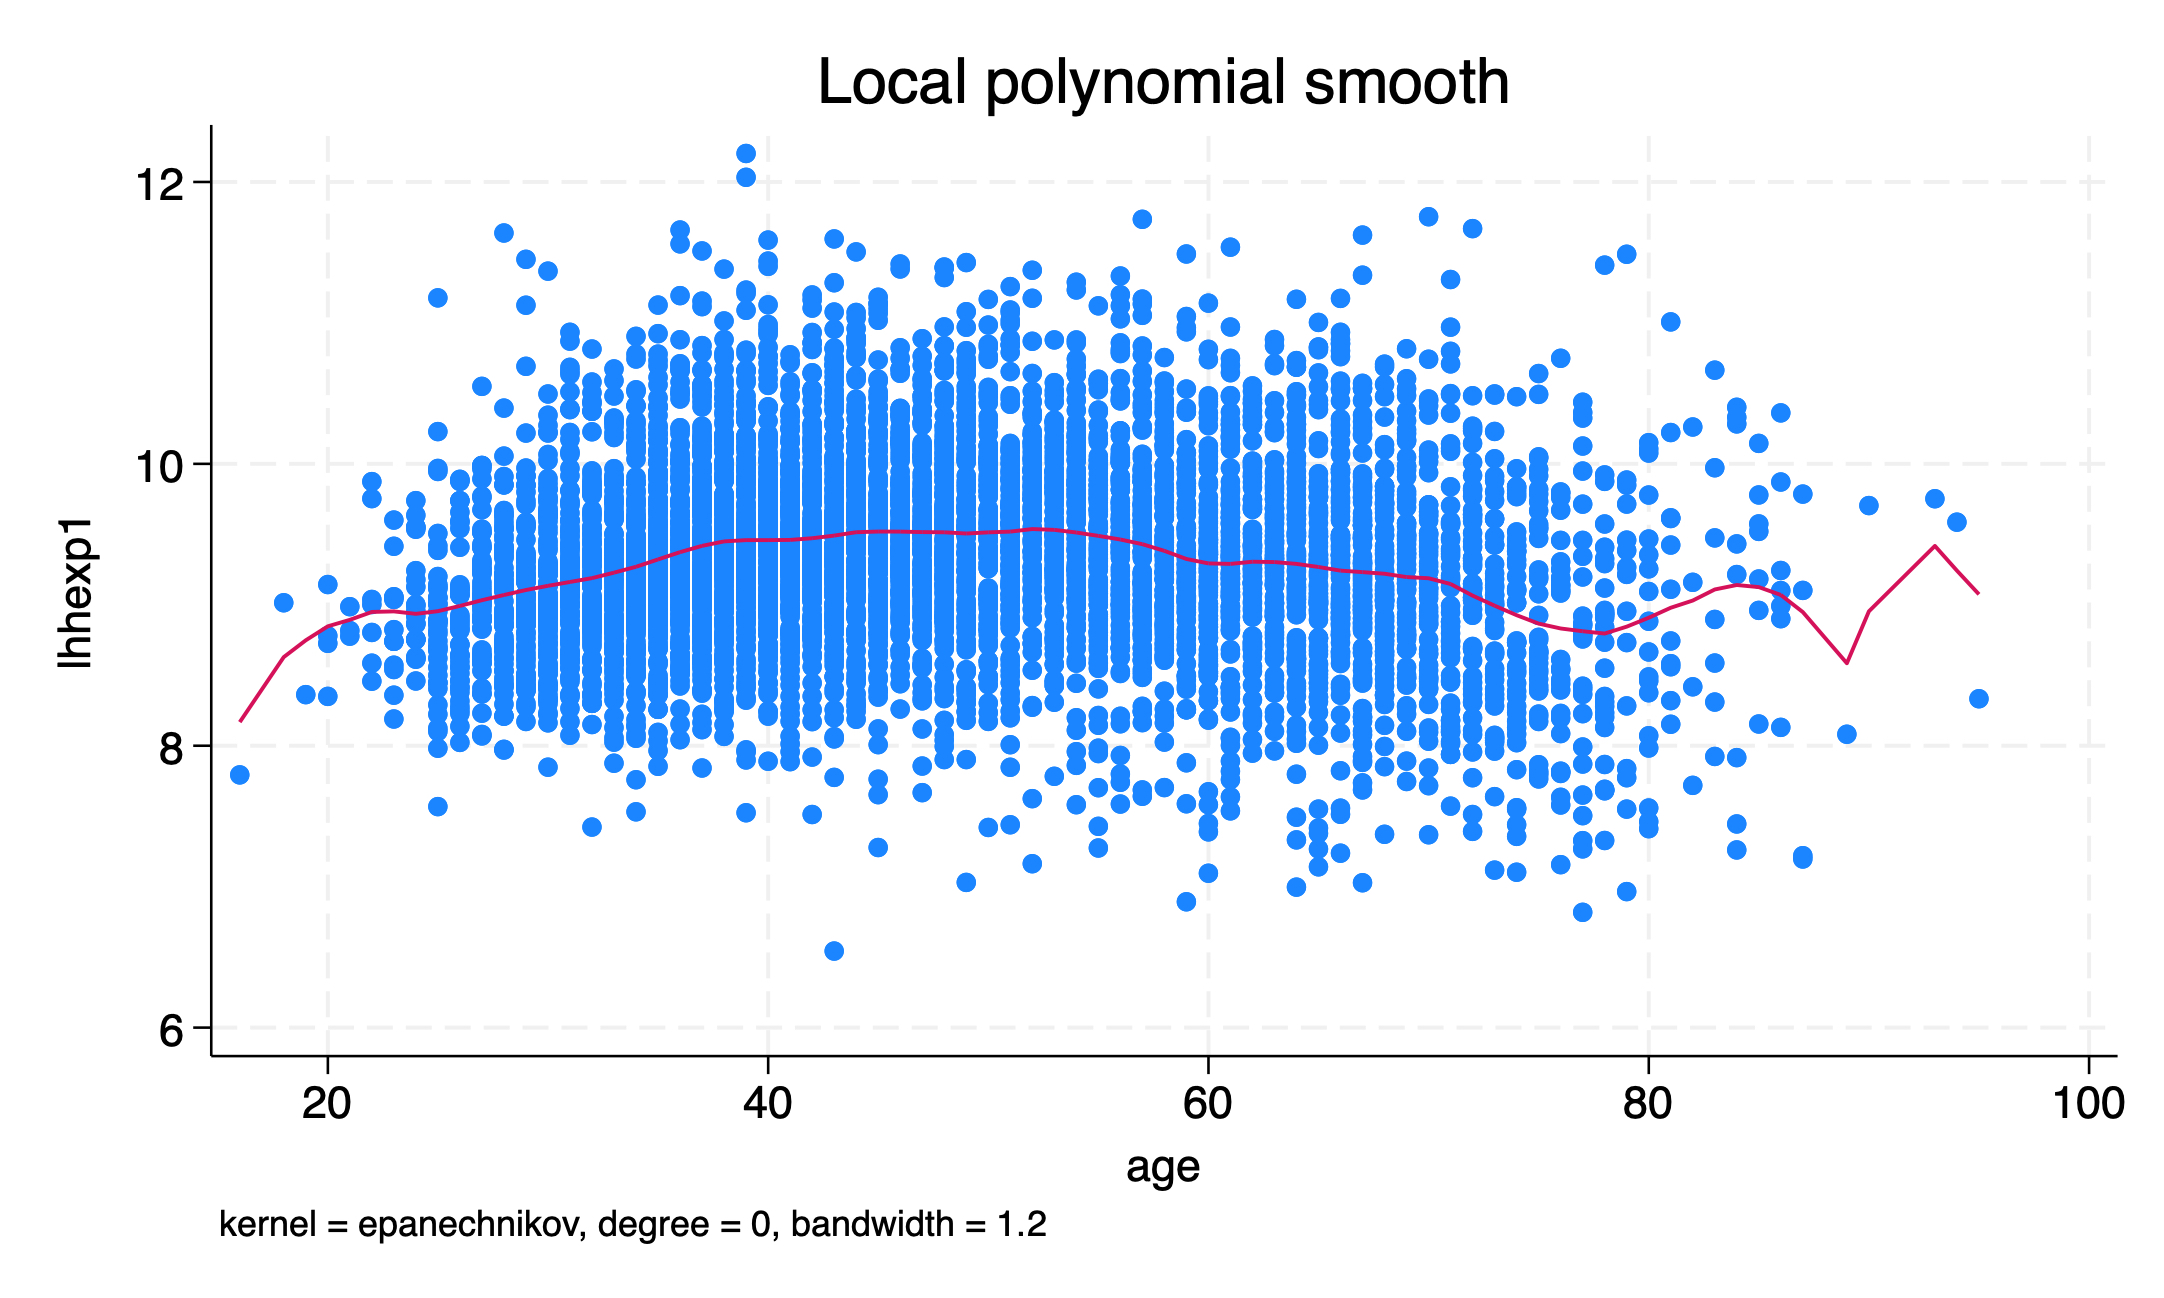
\includegraphics[scale=0.1]{Image/8.jpg}
    \\
    Now we compute the differences.
    \begin{itemize}
        \item \textcolor{Magenta}{gen y= lnrlfood- foodage}
        \item \textcolor{Magenta}{gen x= lhhexp1- expage}
    \end{itemize}
    Finally, we run the regression of y on x, not assuming anything on the distribution
    of the data.\\
    \textcolor{Magenta}{reg y x, noconstant}
    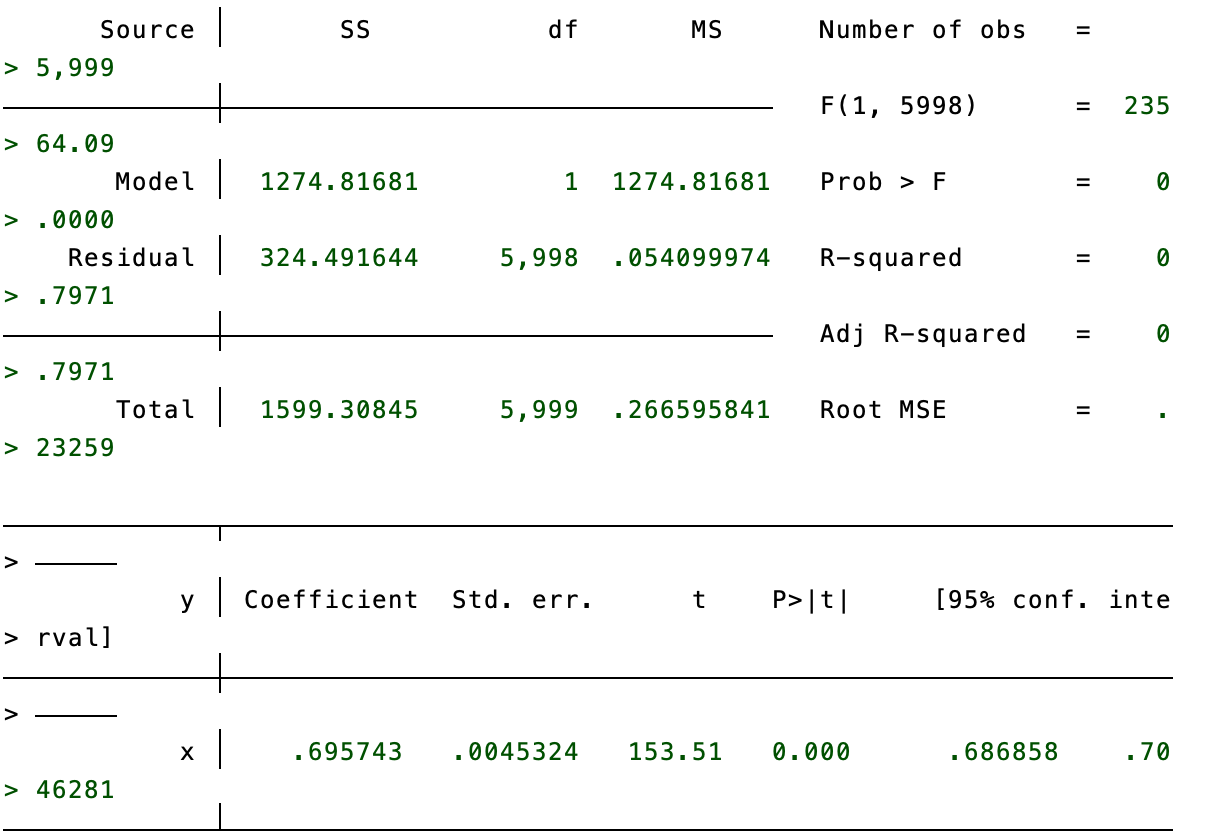
\includegraphics[scale=0.35]{Image/9.png}

\end{homeworkProblem}

\begin{homeworkProblem}
    Compare the results.\\

    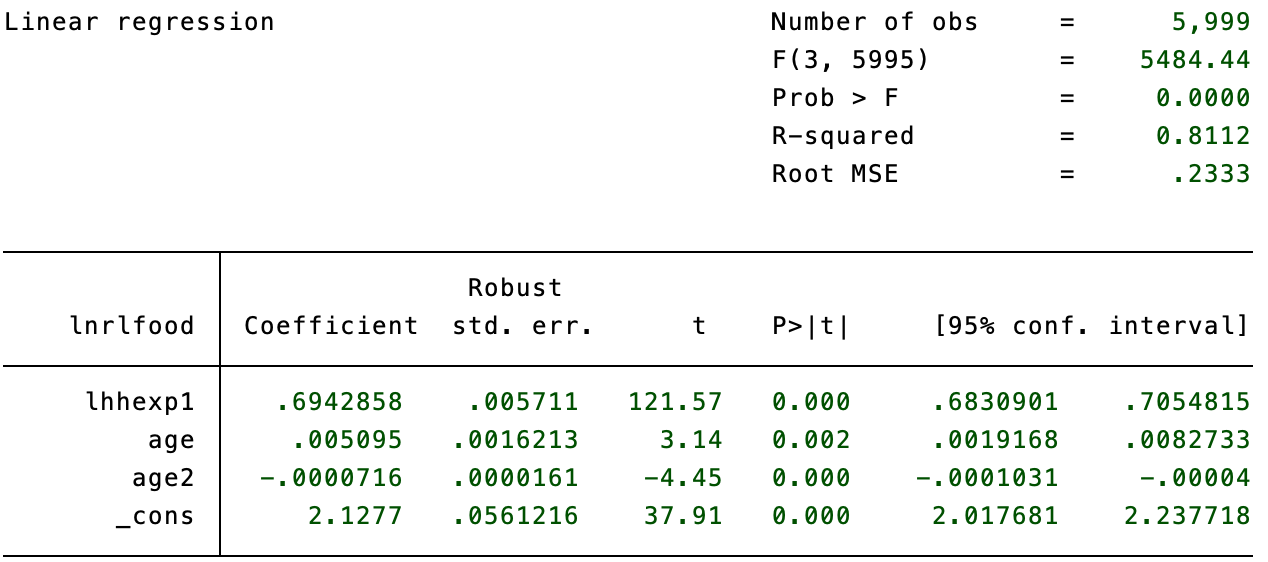
\includegraphics[scale=0.4]{Image/10.png}\\
    Actually quite close.
\end{homeworkProblem}

\end{document}
